\chapter{Implementation}
  This chapter details the implementation of the three main project areas:
  \begin{enumerate}
    \item data collection;
    \item data processing;
    \item classification
  \end{enumerate}
  
  It also provides a graph of a sample recording of each of the activities classified. This process enabled me to better understand the readings recorded during the activities and implement the most useful features at the end.
  
  \section{Data collection}
    This section contains details of the components built to access the accelerometer data and transfer it to a computer.
    
    Because both the smartwatch and the smartphone both run Android, it is possible to create components that are shared between the devices, resulting in less redundancy, less complexity and, ultimately, a more reliable implementation. Both the \texttt{AccelerometerListenerService} and the \texttt{AccelerometerDataBlob} are shared between both devices.
    
    \subsection{Accessing the accelerometer}
      The \texttt{AccelerometerListenerService} is responsible for receiving readings from the accelerometer and delivering them to the data structure responsible for storage.
      
      As described in Section~\ref{sec:sensor-api}, the Sensor API utilises a listener methodology. It is required to create and register a listener that implements \texttt{onSensorChanged()}. 
      
      \subsubsection{Performance considerations}
        Because the accelerometer can update its values at a rate of over 50\si{Hz}, it is vital that any implementation of \texttt{onSensorChanged()} is non-blocking and ideally be very quick to execute. Any expensive computation or IO operation has to be moved to a separate thread.
        
        If the execution of \texttt{onSensorChanged()} takes longer than $\frac{1}{\mathrm{sample-rate}}$, requests for \texttt{onSensorChanged()} will queue and eventually lead to the exhaustion of memory or dropping of data.
        
        For this reason, the data structure used, discussed in Section~\ref{sec:storing-accelerometer-data}, is very lightweight and \texttt{onSensorChanged()} is only responsible for passing data to it.
      
      \subsubsection{Concurrency considerations}
        Because \texttt{onSensorChanged()} can be called at such a high rate, it is possible that new calls to the method can be made while previous calls are still executing. Data corruption could result from improper handling of asynchronicity.
      
        The documentation for the Sensor API is not explicit about whether calls to \texttt{onSensorChanged()} queue on the same thread or whether they can be dispatched asynchronously. For this reason, the \texttt{AccelerometerListenerService} was designed to be thread-safe by using Java concurrency primitives.
      
      \subsubsection{Power consumption considerations}
        Typically, Android will power off the display and later the CPU after a period of user-inactivity. Powering off the CPU means that the device will stop recording accelerometer data, and so it is required to maintain a wake-lock which keeps the CPU from powering off. It is also important to remember to release the wake-lock once accelerometer recording is complete. Otherwise, the device's CPU will remain on even when the device appears to be on standby, using battery. It is for this reason that care should be taken to minimise power usage where possible, while still collecting all the required data.
        
        One tradeoff had to be made between collection strategies. One strategy is to record data at a specified sample rate from when the recording is turned on until it is turned off. An alternative strategy is to record a window of data at set intervals and sleep the remainder of the time. For example, one might set the accelerometer to record 10 seconds of data every 50 seconds.
        
        Though the latter strategy saves battery power as the device turns off the accelerometer between recordings, a continous recording approach was taken in this project in order to have as much data as possible. In addition, the battery life was not severly impeded by the continous recording approach.
        
      \subsubsection{Sampling rate}
        In ideal conditions, it would be sensible to sample at the fastest possible rate: the resultant data can always be downsampled afterwards if it is not required. As per the Nyquist-Shannon sampling theory, discussed in Section~\ref{sec:intro-sig-processing}, our sample rate should be greater than twice the highest frequency of the signal. Because it isn't possible to know what the highest frequency is going to be, it would be reasonable to sample at a far higher rate. 
        
        However, picking a very fast sample rate in this context has two potential downsides: battery life drain and the size of resultant data. I investigated whether either battery life or the size of the resulting data would be a limiting factor of sample rate.
        
        The impact on power consumption when increasing the sample rate was negligible. This may be because the increase in extra work as a result of an increased sample rate is negligable compared to the cost of keeping the CPU awake at all.
      
        Recall from Table~\ref{tab:data-row} that each measurement has a total size of 20 bytes. At a sample rate of 50\si{Hz}, data is produced at approximately 1 KBps or 3.6 MB per hour. The most memory-constrained device is the smartwatch, which only has 512 MB of RAM but 4 GB of internal storage. A data structure that stores the accelerometer data to the internal storage rather than to memory is required, but a sample rate of 50\si{Hz} produces a storable amount of data on any reasonable-length (i.e. up to one hour) activity recording.
        
        Another potential concern regarding data size is the transfer from the smartwatch to the smartphone. The only connection available is Bluetooth. The Bluetooth connection empirically has a maximum transfer rate of no more than 150 KBps, meaning an hour of activity data will take approximately 30 seconds to transfer.

    \subsection{Storing accelerometer data}
      \label{sec:storing-accelerometer-data}
      The data structure to hold the accelerometer data on both the phone and the watch is required to be:
      \begin{itemize}
        \item \textbf{fast} because it will be written to many times per second and cannot block;
        \item \textbf{on-disk} rather than in-memory, because the smartwatch may not have enough free memory to store all the accelerometer data for lengthy recordings;
        \item \textbf{thread-safe} as it is unclear whether calls to \texttt{onSensorChanged()} are queued or concurrent.
      \end{itemize}
      
      The data structure decided on was a temporary random-access file with buffered writing. The data is written as bytes through an output buffer. The output buffer is maintained in memory and is flushed when it reaches capacity. The capacity of the output buffer was set to 20000 bytes as data is only written in multiples of 20 bytes and the smartwatch is comfortably able to keep 20 kb in memory. This equates to data being saved to disk approximately every 20 seconds.
      
      % data structure – binary data
      % local temporary internal storage as opposed to memory
      % delete when transmitted
    \subsection{Transmitting accelerometer data}
      \label{sec:Transmitting_accelerometer_data}
      The accelerometer data has to be transmitted from the smartwatch to the smartphone before it can be transferred to a computer. As discussed in Section~\ref{sec:prep-data-api}, there are two relevant methods to transfer data between the smartwatch and the smartphone: a DataItem and an Asset. Their advantages and disadvantages with respect to this project are highlighted in Table~\ref{tab:dataitem-vs-asset}.
      
      \begin{table}
        \centering
        {\tabulinesep=1.2mm
        \begin{tabu} to \linewidth { X[2,c,m] | X[3,l,m] | X[3,l,m] | }
          & \textbf{DataItem} & \textbf{Asset} \\
          \hline
          \textbf{Advantages} & 
            \begin{itemize}
              \item no separate data fetching step
              \item simpler, more reliable receiver code
              \item negligable transmission time
            \end{itemize} &
            \begin{itemize}
              \item no hard size limit
              \item can create an Asset from a File without storing it in memory
            \end{itemize} \\
          \hline
          \textbf{Disadvantages} &
            \begin{itemize}
              \item 100 KB size limit
              \item have to insert byte arrays
            \end{itemize} &
            \begin{itemize}
              \item some constructors don't seem to work
              \item transmission of large files takes a noticable amount of time
              \item separate data fetching step requires more receiver-side code
            \end{itemize} \\
          \hline
        \end{tabu}}
        \caption{Advantages and disadvantages of using the \texttt{DataItem} and \texttt{Asset} to transmit data from the smartwatch to the smartphone.}
        \label{tab:dataitem-vs-asset}
      \end{table}
      
      Because the DataItem has a 100 KB limit, an alternate transmission and storage system would have to have been built, where the smartwatch collects 100 KB of data and sends that to the smartphone while it continues to record. It is then reassembled at the smartphone receiver.
      
      I consider this solution inferior to the Asset implementation, which allows transmission of any size of data.
      % DataItem has 100kb limit.
      % Bug with Asset class – FileDescriptor
      % Use of Asset transmit
      % Sender
      % Receiver
    \subsection{Mobile apps}
      This section concerns the development of the user-facing components of the application. 
      
      Figure~\ref{fig:app_screenshots} presents screenshots of both the smartphone and smartwatch apps produced.

      \begin{figure}[!th]
        \centering
        \begin{subfigure}[b]{0.3\textwidth}
                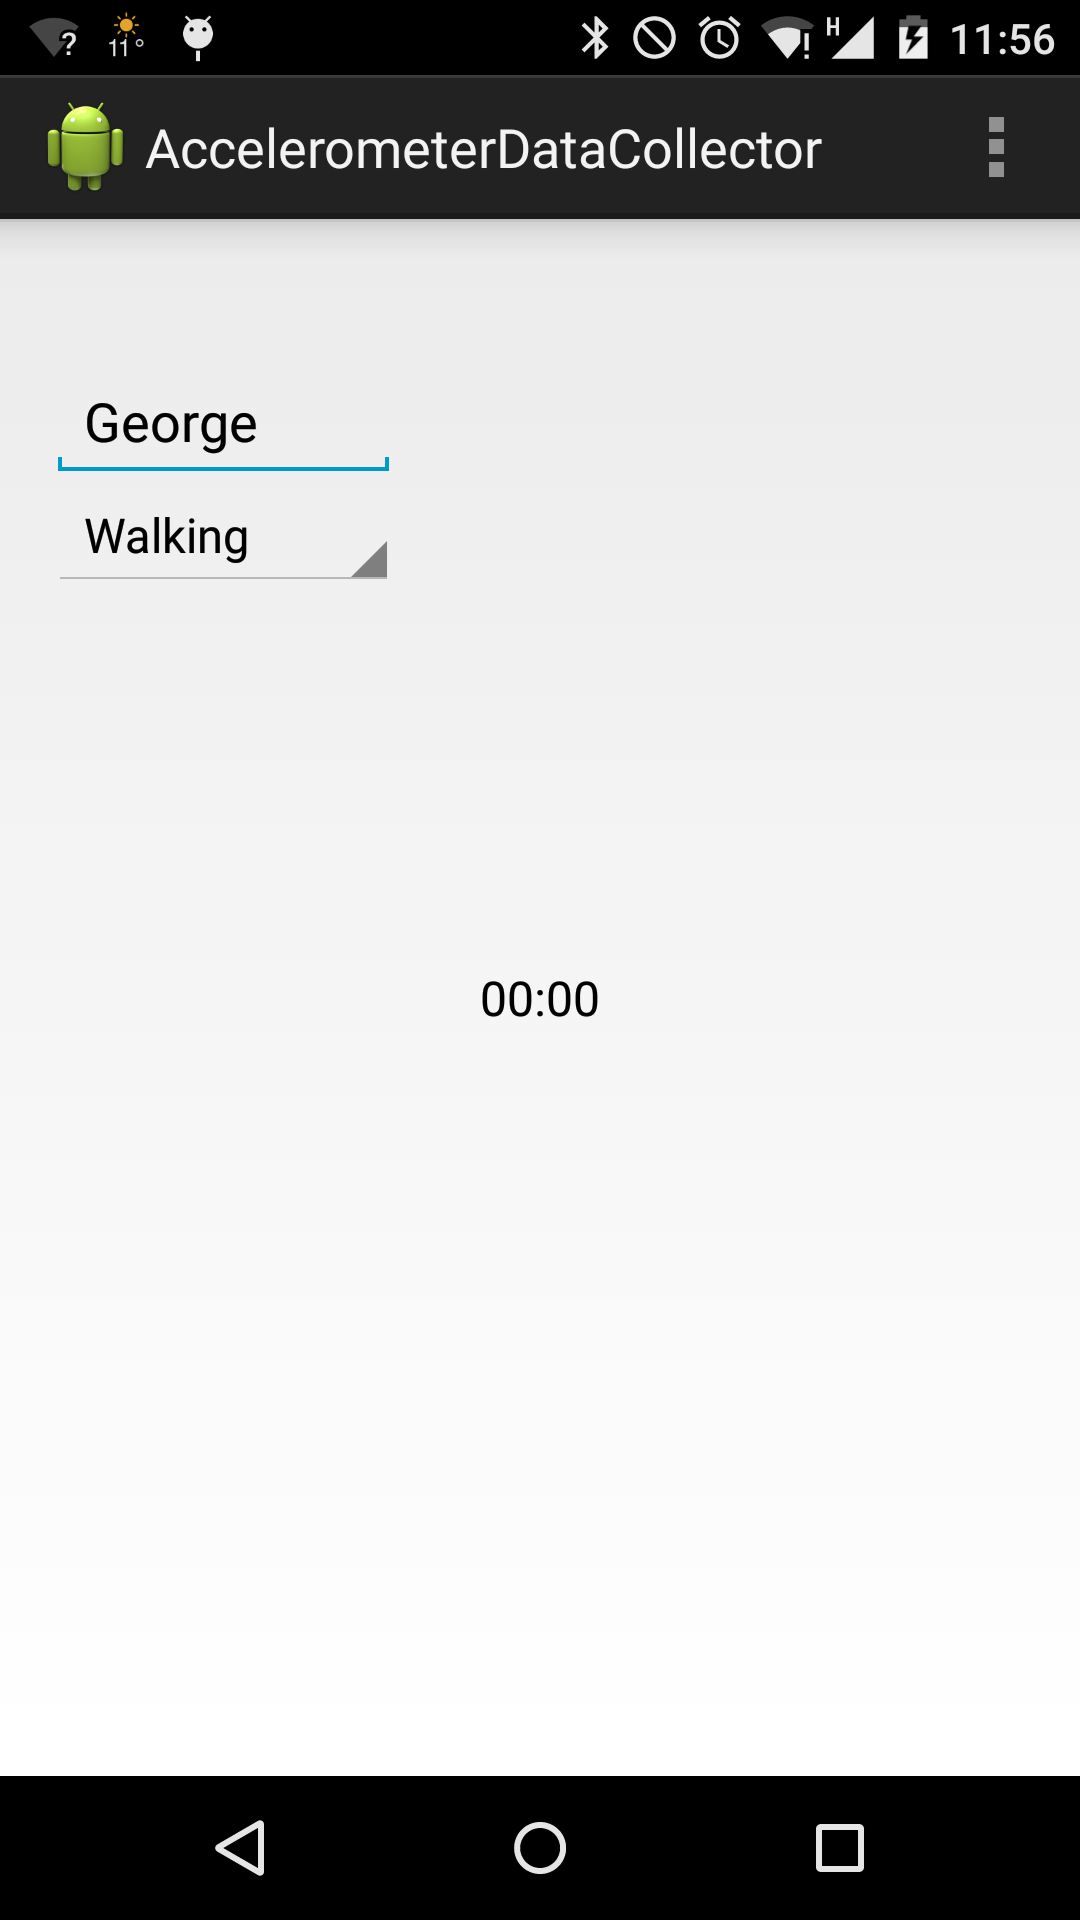
\includegraphics[width=\textwidth]{phone_app_screenshot}
                \caption{The phone app}
                \label{fig:phone_app_screenshot}
        \end{subfigure}
        \qquad
        \begin{subfigure}[b]{0.3\textwidth}
                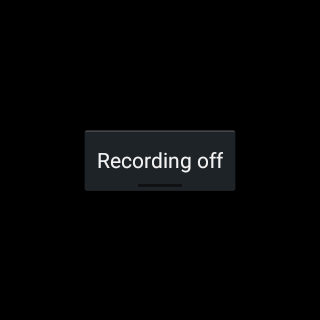
\includegraphics[width=\textwidth]{wear_app_screenshot}
                \caption{The watch app}
                \label{fig:wear_app_screenshot}
        \end{subfigure}
        \caption{Screenshots of the phone and the watch apps}
        \label{fig:app_screenshots}
      \end{figure}
      
      On the smartphone, configuration options are provided on the smartphone. This includes the ability to type a recorder's name and select the activity that is being recorded, which is then included in the recording's filename. A timer is also present, which displays the duration of the current recording so far.
      
      Activity recording is started and stopped from the smartwatch. This is because the smartwatch is typically more accessible than the smartphone, being worn on the wrist rather than left in a pocket. The user is also free to place the phone anywhere before recording starts. This is the only user activity available from the smartwatch.
      
      Figure~\ref{fig:recordingstatemachine} illustrates the state machine which models the recording cycle. A typical recording cycle is thus
      \begin{enumerate}
        \item The user sets their name and the activity they are recording on the phone.
        \item The user begins the recording on the watch.
        \item The watch messages to the phone app, telling it to begin recording.
        \item The phone begins recording.
        \item The user performs the activity.
        \item The user ends recording on the watch.
        \item The watch app messages the phone app, telling it to end recording.
        \item The phone stops recording.
        \item The watch sends its data to the phone, which requires a separate lifecycle:
        \begin{enumerate}
          \item The watch messages the smartphone indicating there is data to transfer.
          \item The phone sets up the transfer of the data from the watch.
          \item The phone saves the data from the watch.
        \end{enumerate}
        \item The phone also saves its own data.
      \end{enumerate}
      
      \begin{figure}[!th]
        \centering
        \begin{tikzpicture}[>=stealth',shorten >=1pt,auto,node distance=4cm]
          \node[initial,state] (S)                {$\bar{p}\bar{w}$};
          \node[state]         (q1) [right of=S]  {$\bar{p}w$};
          \node[state]         (q2) [below of=q1] {$pw$};
          \node[state]         (q3) [below of=S]  {$p\bar{w}$};

          \path[->] (S) edge           node {start button} (q1)
                (q1) edge              node {message} (q2)
                (q2) edge              node {stop button} (q3)
                (q3) edge              node {message} (S);
        \end{tikzpicture}
        \caption[A state machine of the recording cycle]{A state machine of the recording cycle. $p$ and $w$ indicate that the phone and watch are recording respectively. Message passing is implemented through the Android Wear API.}
        \label{fig:recordingstatemachine}
      \end{figure}
      
      A decision that had to be made was whether it was required for the recordings to start at precisely the same time, as the message parsing between the watch and the phone to signal the start of the recording is fast but it is not instant. 
      
      Recordings starting at exactly the same time mean that it may be easier to correlate movements between devices, but it this doesn't seem to be particularly useful if the message parsing means the records start within microseconds of each other and cross-correlation may be able to help align them completely.  
      
  \section{Activity analysis}
    \label{sec:activity-details}
    The apps were used to collect data over a range of activities. This section provides the graphs of the magnitude and the Fourier transform of the magnitude. I used these graphs to better understand the accelerometer readings resulting from different activities and justify the utility of the features I hope to extract from the data.
    
    For each activity, I graph an arbitrary ten second snippet as recorded by both the phone and watch. The ten second snippet has been low-pass filtered with a critical frequency of 5Hz, as described in Section~\ref{sec:preprocessing}. The Fourier transform for the same snippet is also provided, so as to display the recording in the frequency domain as well as the time domain.
    
    For all recordings, the watch was worn tight on the non-dominent left hand and the phone was kept in the right side trouser pocket.
    
    Recall from Section~\ref{sec:activities_for_classification} the activities I picked to classify:
    \begin{itemize}
      \item Physical activities requiring whole body motion:
      \begin{itemize}
        \item Climbing
        \item Cycling
        \item Gym cycling
        \item Running
        \item Stair climbing
        \item Walking
      \end{itemize} 
      \item Activities that primarily require arm motion:
      \begin{itemize}
        \item Computer use
        \item Eating
        \item Playing fussball
      \end{itemize}
      \item Low energy upright activities:
      \begin{itemize}
        \item Gallery perusal
        \item Standing
        \item Teeth brushing
      \end{itemize}
    \end{itemize}
    \pagebreak[4]
    \subsection{Climbing}
      \begin{figure}[!th]
        \centering
        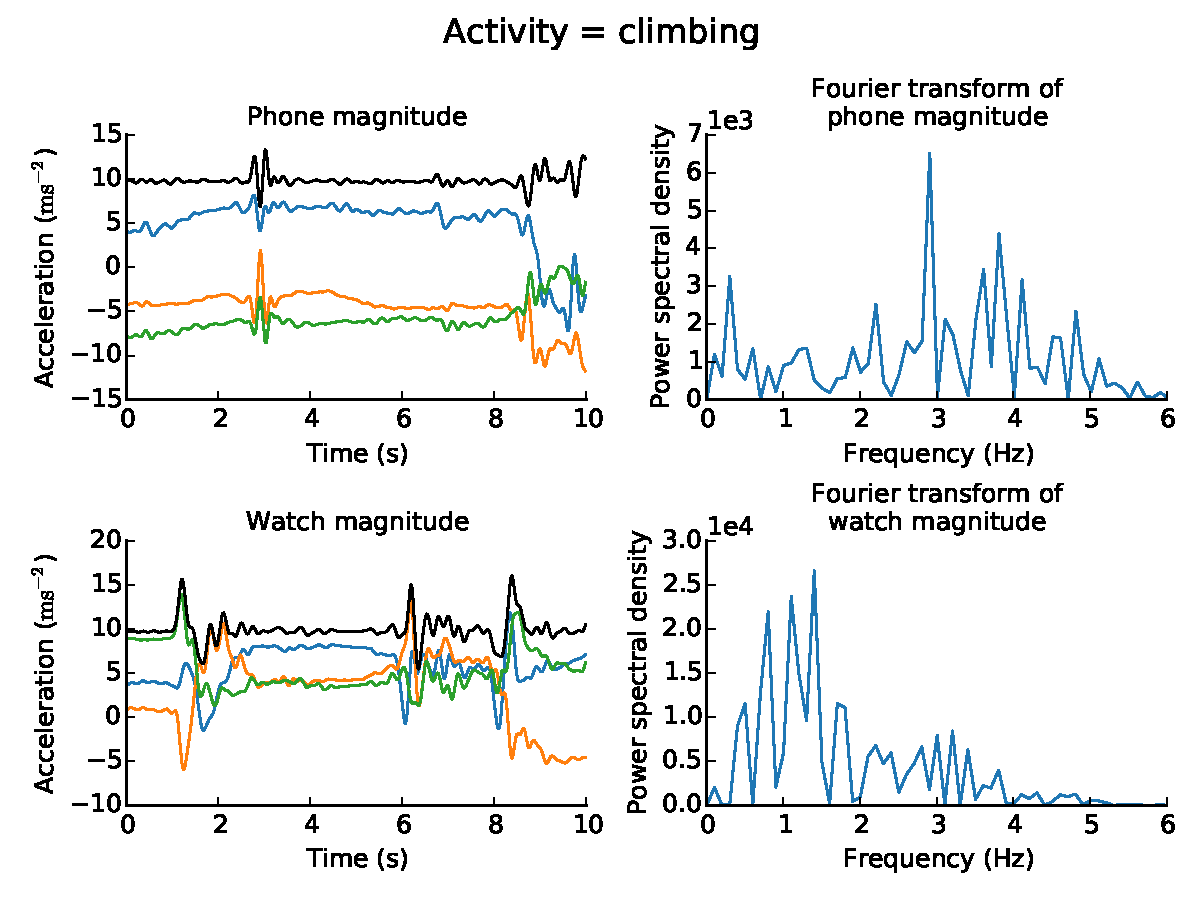
\includegraphics[width=0.8\textwidth]{2by2climbing}
        \caption[Climbing sample]{Ten seconds of phone and watch data from a climbing activity together with their Fourier transforms.}
        \label{fig:2by2climbing }
      \end{figure}
      
      I recorded a session of indoor bouldering, which is climbing on short walls with no ropes.
      
      Climbing has no period or pattern, as movement is wholly dependent on the routes being climbed. Magnitude of acceleration is unpredicable: moves can be made quickly or slowly.
      
      
    \pagebreak[4]
    \subsection{Computer use}
      \begin{figure}[!th]
        \centering
        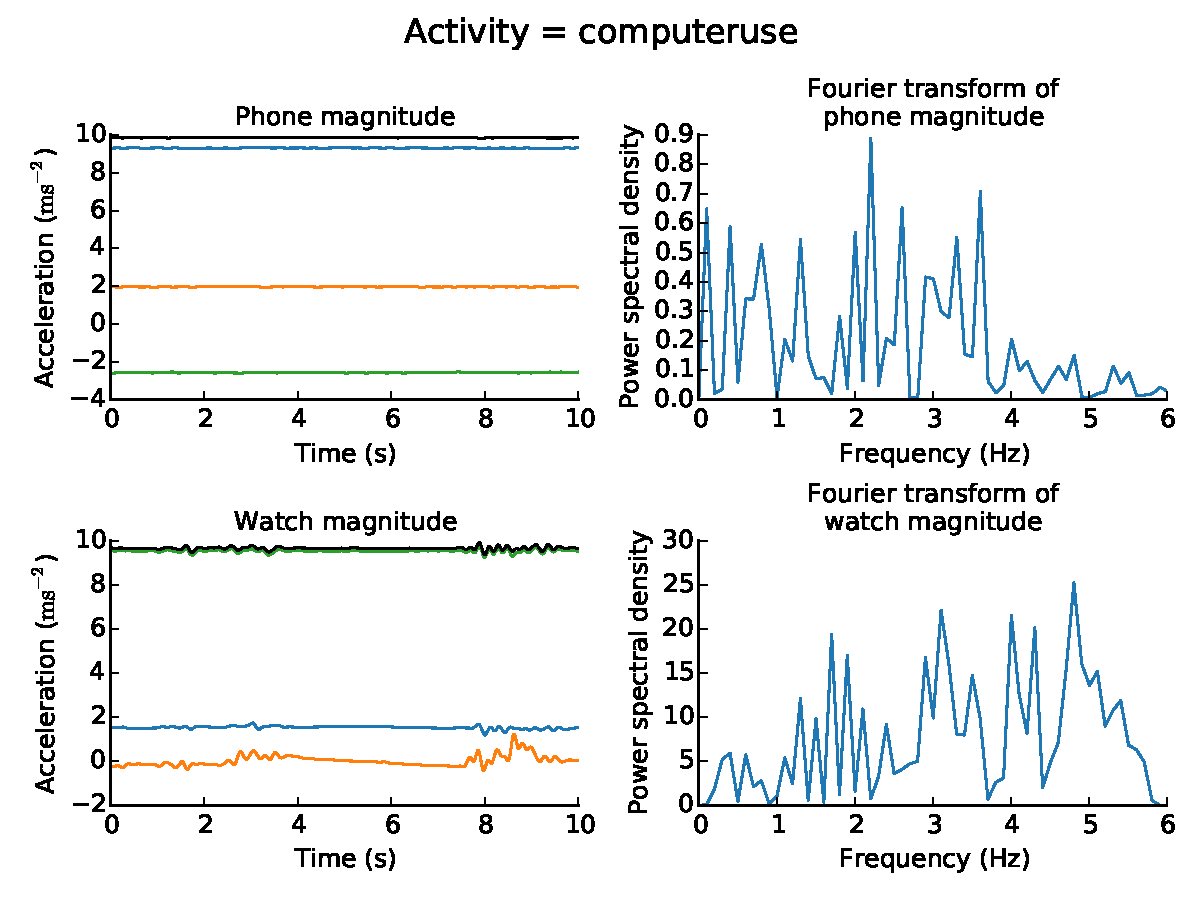
\includegraphics[width=0.8\textwidth]{2by2computeruse}
        \caption[Computer use sample]{Ten seconds of phone and watch data from a computer use activity together with their Fourier transforms.}
        \label{fig:2by2computeruse}
      \end{figure}
      
      Computer use is predominently typing or using a laptop trackpad while seated. The watch was worn on the left, non-dominant wrist while the phone was kept in the right trouser pocket. There is very little movement in the phone, as the leg is mostly stationary. The watch exhibits some periodic movement punctuated by periods of inactivity. This is presumably from typing a word and then pausing.
      
      The Fourier transform of the watch magnitude indicates that watch movement is also aperiodic, as one might expect from typing with frequent pauses. 
    \pagebreak[4]
    \subsection{Cycling}
      \begin{figure}[!th]
        \centering
        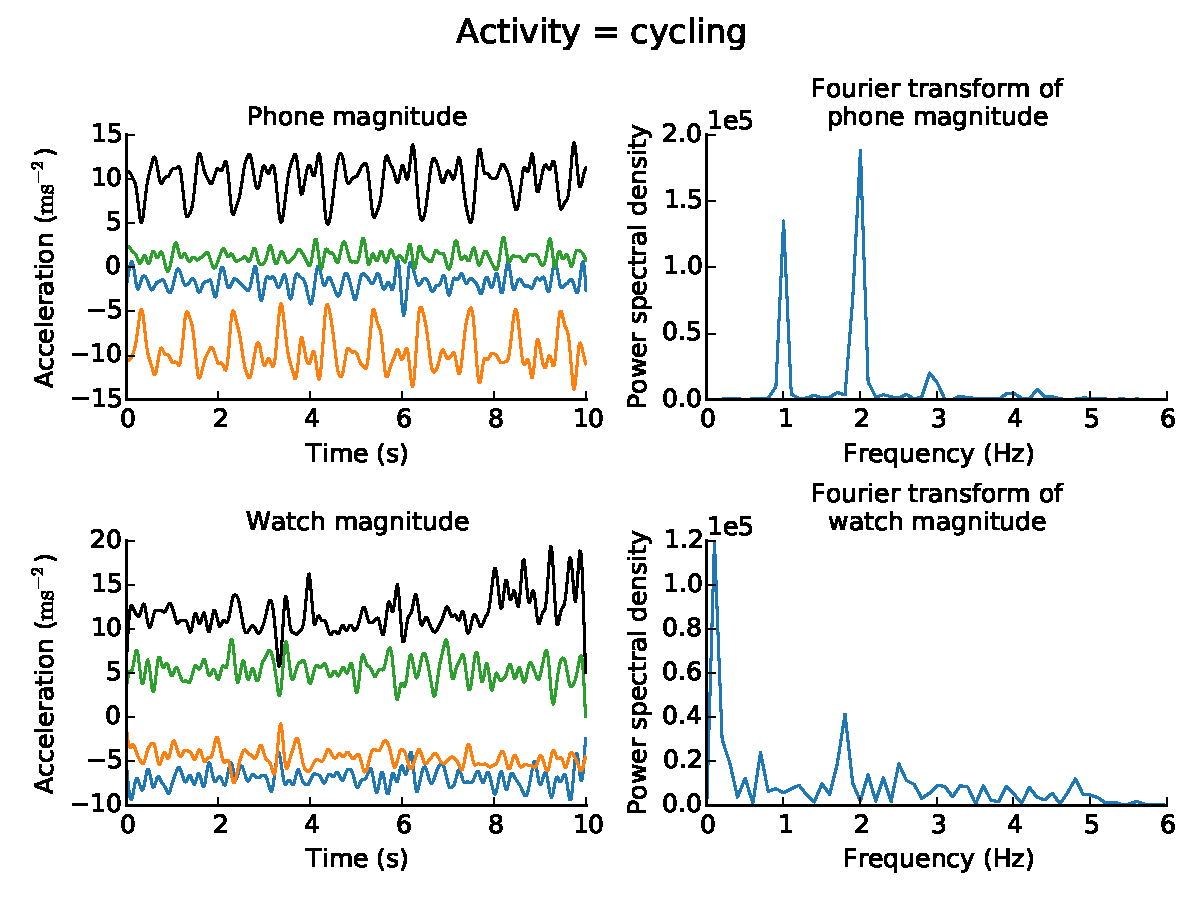
\includegraphics[width=0.8\textwidth]{2by2cycling}
        \caption[Cycling sample]{Ten seconds of phone and watch data from a cycling activity together with their Fourier transforms.}
        \label{fig:2by2cycling}
      \end{figure}
      Cycling is another activity with high periodicity in the phone measurement, but, unlike walking, does not have much periodicity in the watch measurement. This is primarily because of the changing position on the handlebars.
    \pagebreak[4]
    \subsection{Gym cycling}
      \begin{figure}[!th]
        \centering
        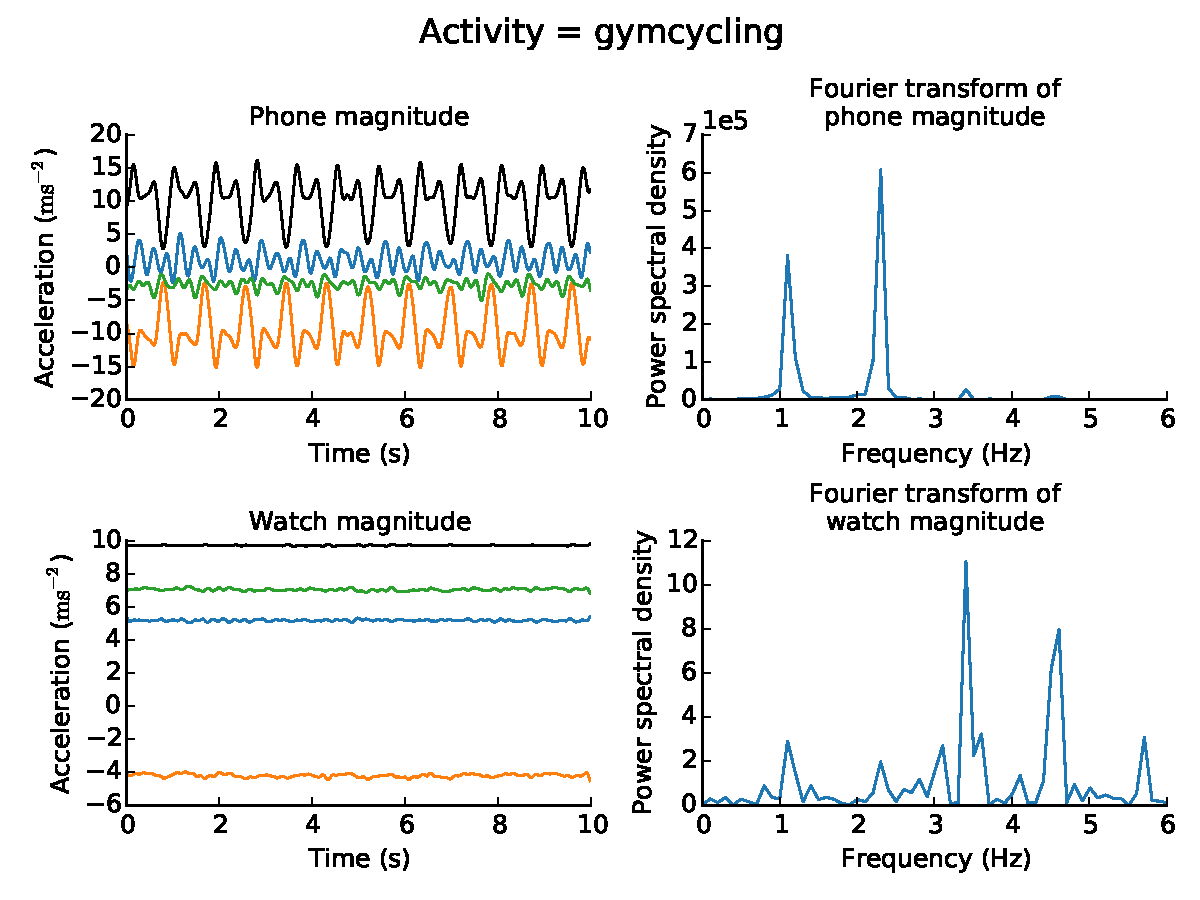
\includegraphics[width=0.8\textwidth]{2by2gymcycling}
        \caption[Gym cycling sample]{Ten seconds of phone and watch data from a gym cycling activity together with their Fourier transforms.}
        \label{fig:2by2gymcycling}
      \end{figure}
      
      Gym cycling is cycling performed on a fixed cycling machine, as opposed to a bike in the real world.
      
      Compared to cycling outdoors, gym cycling has little wrist movement and is more starkly periodic in the phone measurement, as the peddaling action is much more consistent. There is also a lack of linear acceleration in the gym which is present outdoors. Outdoor cycling is often subject to stopping and starting.
      
      Both types of cycling activity would benefit from anaylsis of the top two frequencies of maximum power, at they both exhibit very strong peaks at $1 \si{Hz}$ and $2 \si{Hz}$.
    \pagebreak[4]
    \subsection{Eating}
      \begin{figure}[!th]
        \centering
        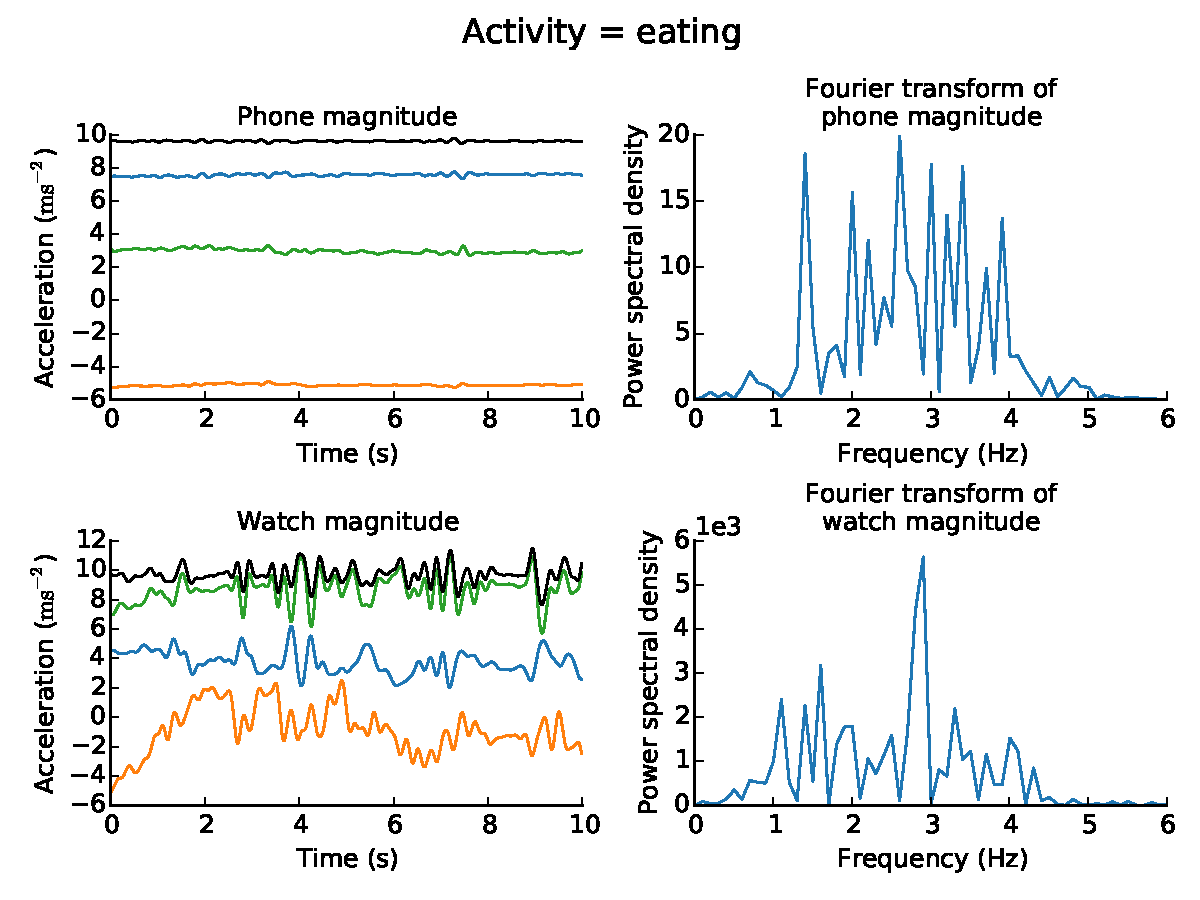
\includegraphics[width=0.8\textwidth]{2by2eating}
        \caption[Eating sample]{Ten seconds of phone and watch data from an eating activity together with their Fourier transforms.}
        \label{fig:2by2eating}
      \end{figure}
      
      Eating is a seated activity, so shares much of the phone data with something like computer use, again assuming the phone is in the right trouser pocket. The watch data has more energy, but is aperiodic.
      
      A feature that distinguishes amount of movement in the watch should be able to distinguish between eating and computer use activities.
    \pagebreak[4]
    \subsection{Playing fussball}
      \begin{figure}[!th]
        \centering
        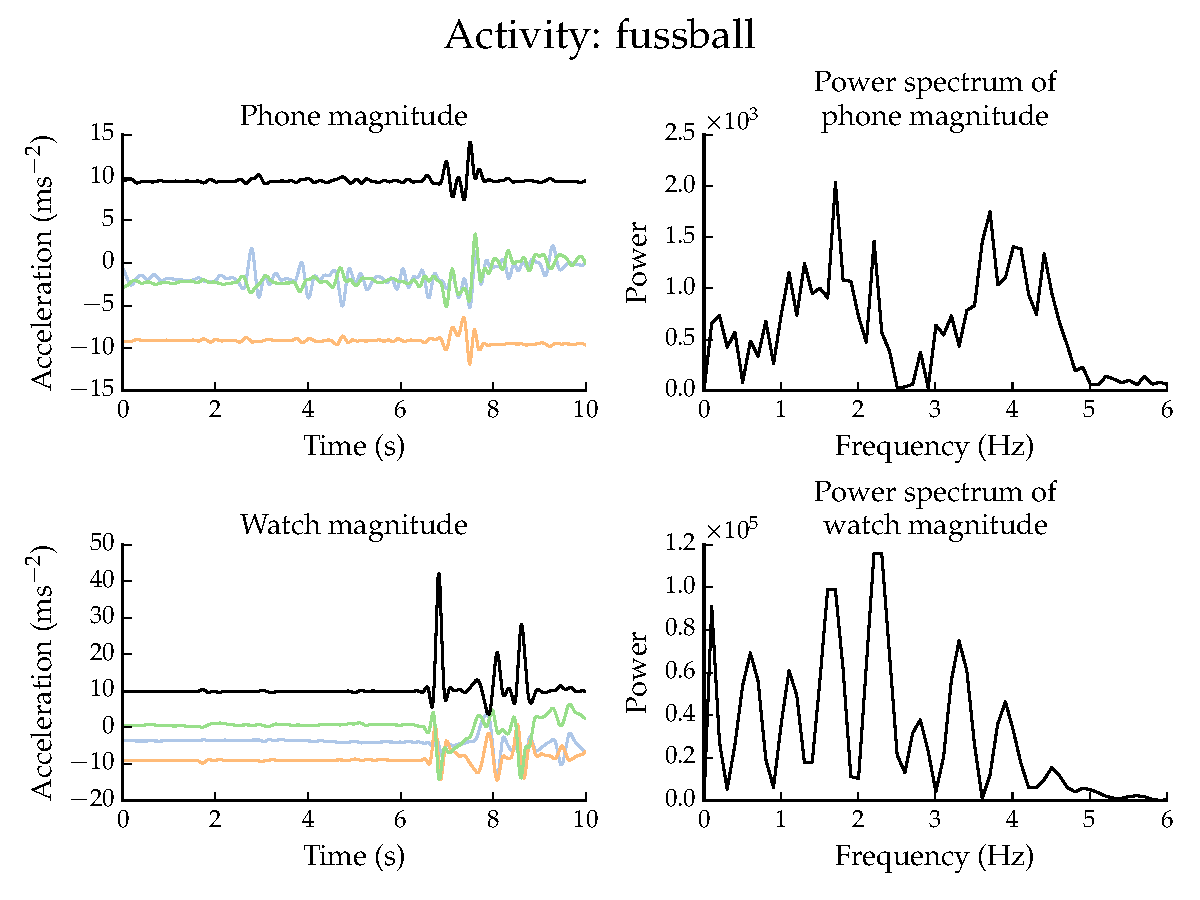
\includegraphics[width=0.8\textwidth]{2by2fussball}
        \caption[Fussball sample]{Ten seconds of phone and watch data from a fussball activity together with their Fourier transforms.}
        \label{fig:2by2fussball}
      \end{figure}
      
      Fussball (also known as table football) is characterised by periods of inactivity followed by sharp acceleration in the watch measurement. The maximum of the magnitude should in theory differentiate this activity from others.
      
      However, the maximum is by definition a statistic that is highly sensitive to outliers and so other activities may exhibit a similarly high magnitude even if it is not characteristic of that activity. A better metric might be a count of the number of data points that exceed a certain thereshold magnitude e.g. $40 \si{\metre\per\square\second}$ 
    \pagebreak[4]
    \subsection{Gallery perusal}
      \begin{figure}[!th]
        \centering
        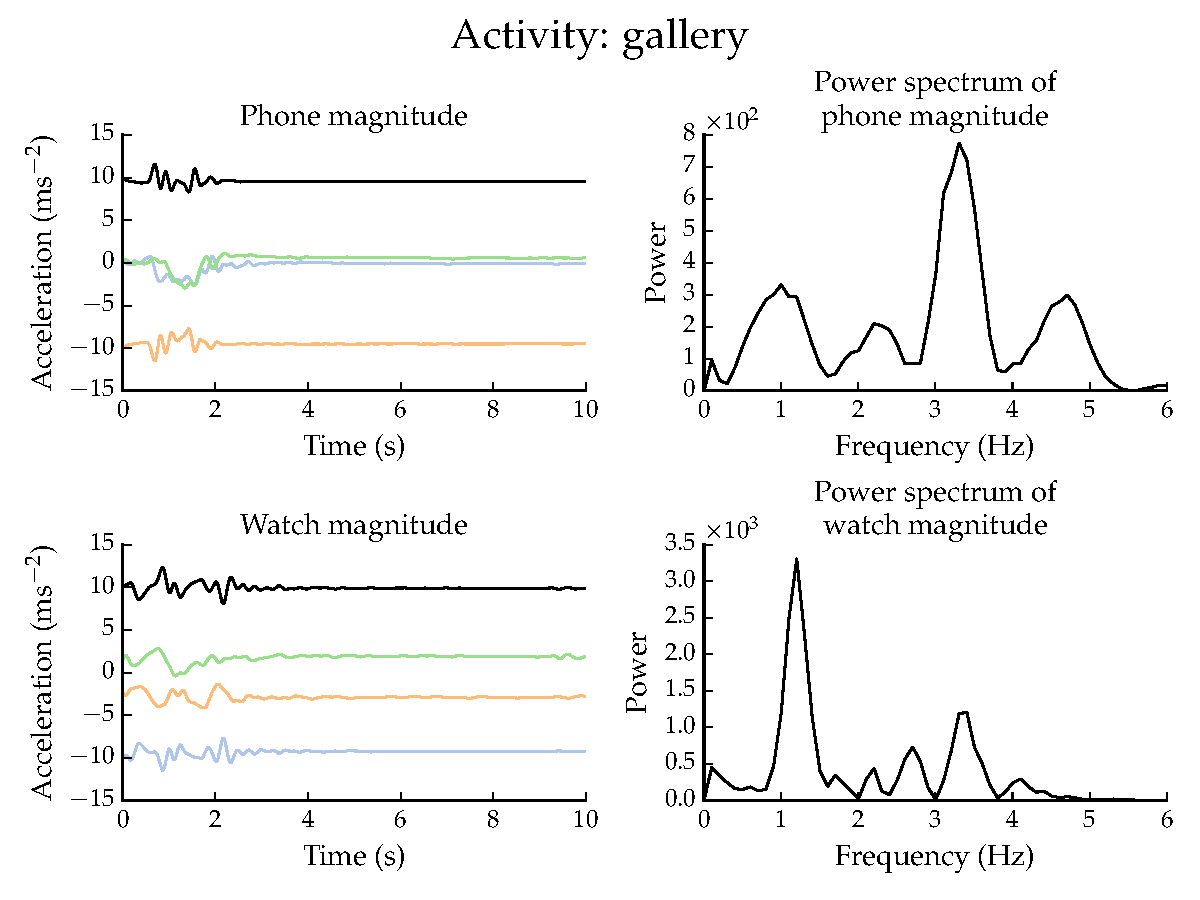
\includegraphics[width=0.8\textwidth]{2by2gallery}
        \caption[Gallery perusal sample]{Ten seconds of phone and watch data from a gallery perusal activity together with their Fourier transforms.}
        \label{fig:2by2gallery}
      \end{figure}
      
      I recorded data while viewing a gallery exhibition. Gallery perusal presents a unique combination of slow walking and standing.
      
      A good classifier would therefore recognise that both walking and standing were present in the recording and classify it as a gallery viewing activity instead.
    \pagebreak[4]
    \subsection{Running}
      \begin{figure}[!th]
        \centering
        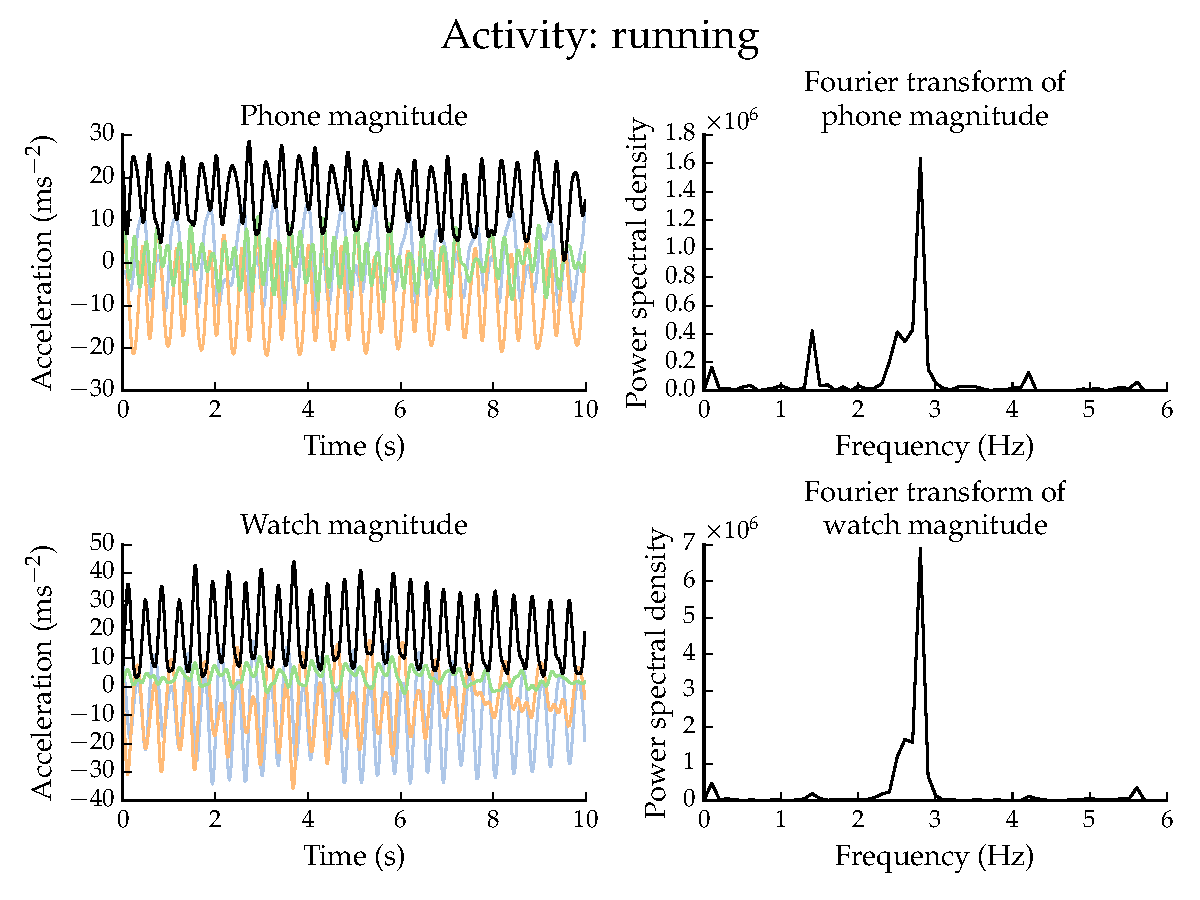
\includegraphics[width=0.8\textwidth]{2by2running}
        \caption[Running sample]{Ten seconds of phone and watch data from a running activity together with their Fourier transforms.}
        \label{fig:2by2running}
      \end{figure}
      
      Running was performed outdoors. Running has a strong period in both the watch and the phone at a frequency which is slightly higher than of walking.
      
      An analysis of the frequency of maximum amplitude may be suffient to classify this activity, though it might be necessary to deterimine how much bigger the peak is than the rest of the power spectrum.
      
    \pagebreak[4]
    \subsection{Stair climbing}
      \begin{figure}[!th]
        \centering
        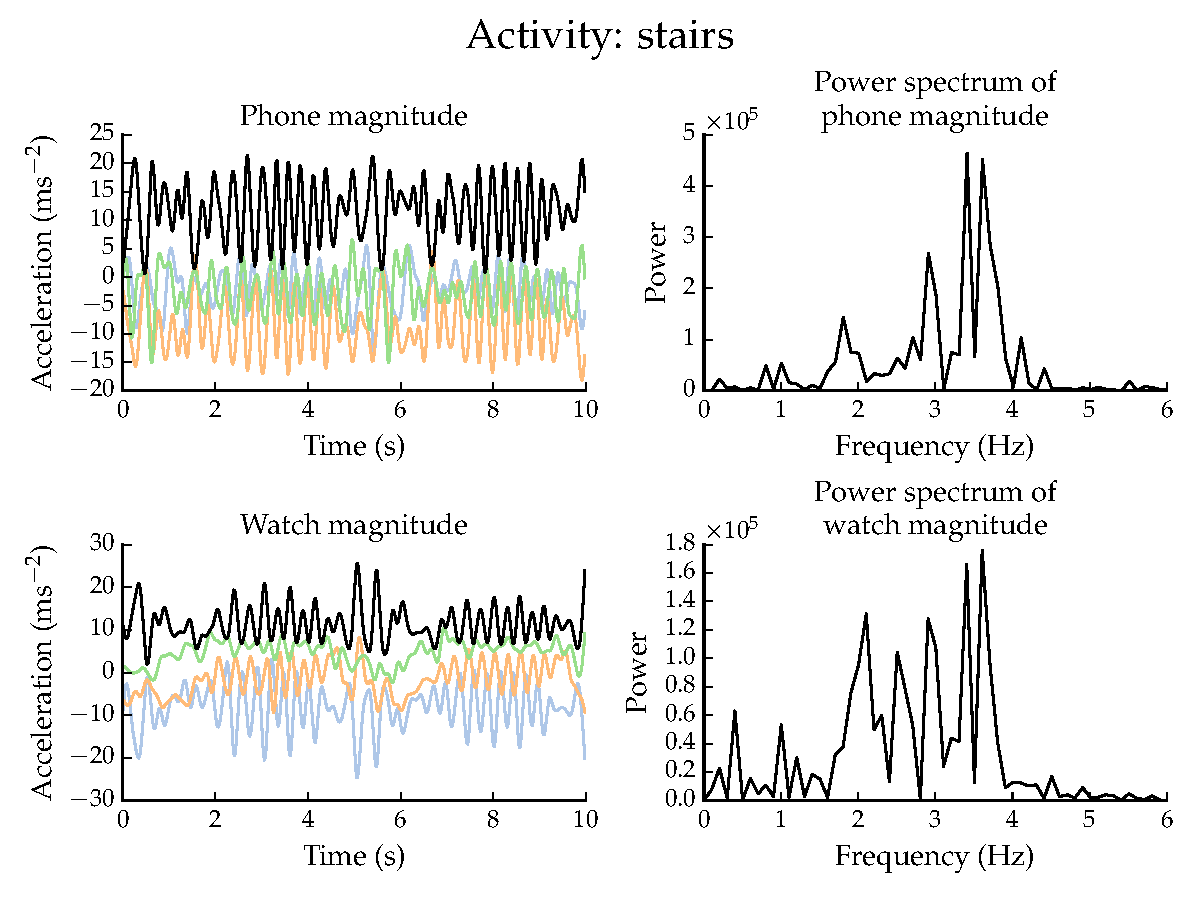
\includegraphics[width=0.8\textwidth]{2by2stairs}
        \caption[Stair climbing sample]{Ten seconds of phone and watch data from a stair climbing activity together with their Fourier transforms.}
        \label{fig:2by2stairs}
      \end{figure}
      Stairs were climbed in the computer lab. A single recording contains climbing and descending stairs. Stairs were climbed either one at a time or two at a time, with the hand either loose or holding the handrail.
      
      This means that stair climbing exhibits a variety of frequencies --- descending stairs is typically done a much quicker pace than climbing stairs, for example. This particular example seems to be drawn from stair descending.
      
      Stairs can be differentiated from walking by noting that though there are still definite periods apparant in the Fourier transform, the peaks are not quite as clear as they are while walking.
    \pagebreak[4]
    \subsection{Standing}
      \begin{figure}[!th]
        \centering
        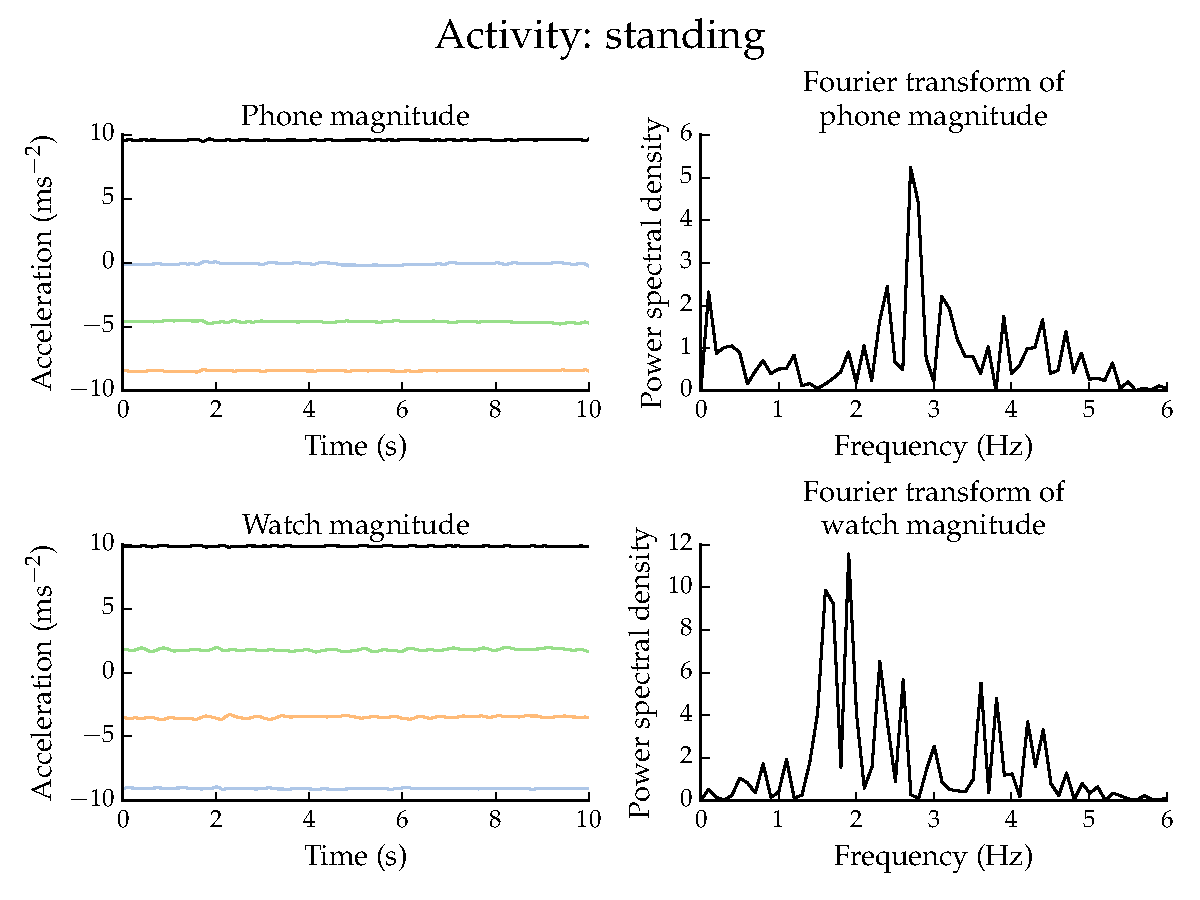
\includegraphics[width=0.8\textwidth]{2by2standing}
        \caption[Standing sample]{Ten seconds of phone and watch data from a standing activity together with their Fourier transforms.}
        \label{fig:2by2standing}
      \end{figure}
      Standing as an activity exists to test differentiation between other upright activities such as toothbrushing and fussball. The phone is largely stationary while the watch moves between certain key standing positions (e.g. arm hanging, in pocket, on hip etc.). 
      
      The mean and the standard deviations of the x, y, and z axes of the phone will show standing activities. Standing exhibits less periodicity than teeth brushing and exhibits less magnitude than fussball, but this magnitude may only be seen in the watch.
    \pagebreak[4]
    \subsection{Teeth brushing}
      \begin{figure}[!th]
        \centering
        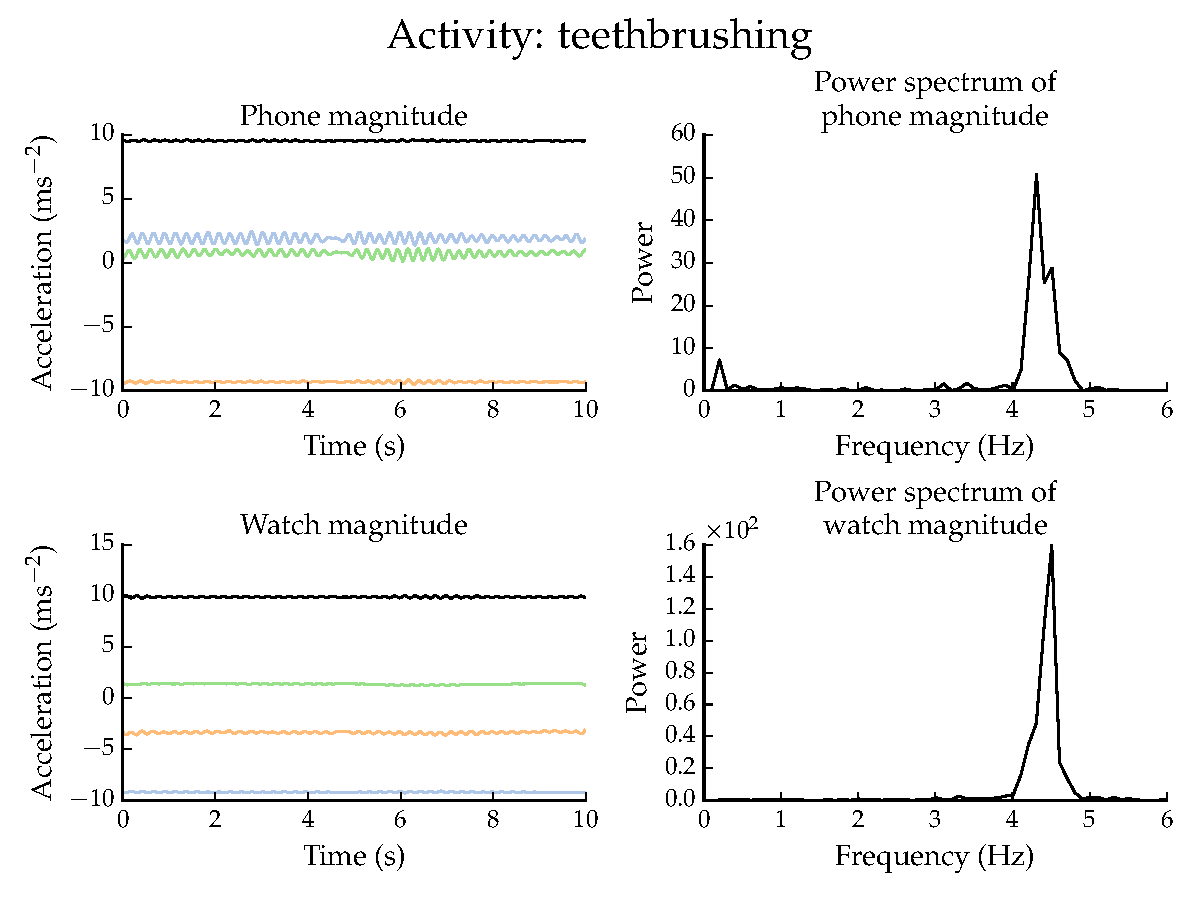
\includegraphics[width=0.8\textwidth]{2by2teethbrushing}
        \caption[Teethbrushing sample]{Ten seconds of phone and watch data from a toothbrushing activity together with their Fourier transforms.}
        \label{fig:2by2teethbrushing}
      \end{figure}
      
      Teeth brushing is conducted with my dominant right hand, while the watch is worn on the left. The phone remains in the right hip pocket. The left hand is often left hanging or resting on the sink. Nevertheless, quite a clear peak is seen on both the watch and the phone recordings of teeth brushing.
      
      Note that this peak is not likely to appear had the teeth brushing be conducted with an electric toothbrush.
      
      As the only activity with a peak in the $4 \sim 5 \si{Hz}$ range, it should be easy to distinguish from other activities such as standing.
    \pagebreak[4]
    \subsection{Walking}
      \begin{figure}[!th]
        \centering
        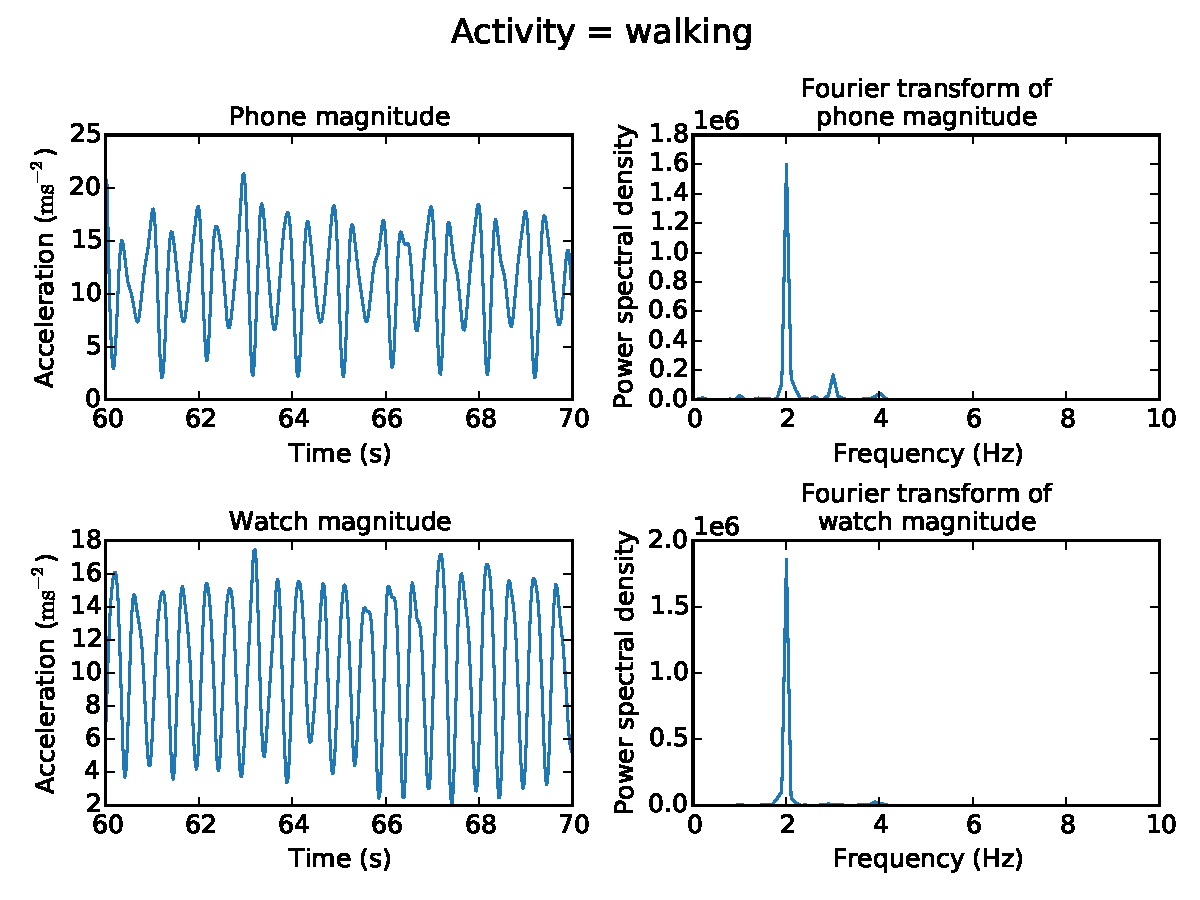
\includegraphics[width=0.8\textwidth]{2by2walking}
        \caption[Walking sample]{Ten seconds of phone and watch data from a walking activity together with their Fourier transforms.}
        \label{fig:2by2walking}
      \end{figure}
      
      Walking is among the most periodic of all the activities investigated. There is a very strong peak at about 2 Hz -- a typical walking pace. There are smaller local maxima at 1, 3 and 4 Hz in the Fourier transform of the phone magnitude, and peaks at 2 Hz and 4 Hz in the watch magnitude. The rest of the Fourier transform is relatively flat.
      
      A useful feature for distinguishing between activies that exhibit strong periodicity is the spectral flatness measure, discussed in Section~\ref{sec:feature-extraction}.

  \section{Data processing}
    \label{sec:data-processing}
    As explained in Section~\ref{sec:programming_languages}, the data processing pipeline was written in Python, because of the strength of its numerical, statistical and machine learning libraries. The data processing was done on a computer as opposed to directly on the phone for two reasons:
    \begin{itemize}
      \item the computational and memory demand of training a classifier; and
      \item data processing and extracting features post-hoc permits me to explore different features from the raw data. Feature extraction is a distructive process and so conducting it on-device means I cannot then extract further features in the future. This goes against the agile development methodology.
    \end{itemize}
    
    Extracting features on the watch and the phone would have had one potential upside: the volume of data required to store and to send is greatly reduced. 
    
    If this were to be developed for wider use, one might consider using a cloud server for classification.
  
    \subsection{Importing and preprocessing}
      \label{sec:importing-and-preprocessing}
      \subsubsection{Import}
        Each recording is stored in a separate binary file. The filename is always of the form: \texttt{<timestamp>-<recorder>-<device>-<activity>.dat}
        
        NumPy includes methods to specify the types of binary data in a file and create an array from it. These are used to great effect to convert the binary data back into longs and floats.
        
        Data files are then accessed via a SQLite database, using the timestamp as the unique ID. The database allows easier access to individual records and, for example, all recordings of a certain activity.
        %read bytes
        %database
      \subsubsection{Preprocessing}
        \label{sec:preprocessing}
        Data is preprocessed before feature extraction.
        
        The first step is the drop the first and last 10 seconds of each data recording. This step is justified as these parts of the accelerometer recordings will not actually be representative of the activity to be classified. Rather, they will primarily be recording the starting and ending of an activity.
        
        For each data recording, the magnitude of the acceleration $\|\mathbf{x}\| = \sqrt{x^2+y^2+z^2}$ was calculated. Patterns in the magnitude were found to be more distinguishing than any of the features extracted from the three axes individually. The magnitude is orientation-invariant, which gives better results when considering that a wrist may move in the same way but may be oriented slightly differently. In this scenario, periodicity will still be observed in the magnitude but may not be observed in each of the three axes individually.
        
        Data is then filtered. As discussed in Section~\ref{sec:intro-sig-processing}, the data recorded by the accelerometer is subject to noise. Reducing the effect of this noise will produce a signal in which it is easier to observe the underlying patterns produced by movement.
        
        A fifth-order Butterworth Filter with a critical frequency of 5~  \si{Hz} was used in order to achieve this. The Butterworth Filter was chosen because it has no gain ripple in the pass band or the stop band. The slow cutoff is not a problem for the application, as the frequencies of activities concerned are far less than the frequency of the noise. A graph of the frequency responses for several Butterworth Filters is given in Figure~\ref{fig:butterworth_filters}.
        
        The frequency response $G(\omega)$, or gain, of an $n$th-order Butterworth filter whose critical frequency is 1 \si{Hz} is:
        
        $$G(\omega) = \sqrt(\frac{1}{1+\omega^{2n}})$$
        
        \begin{figure}
          \centering
          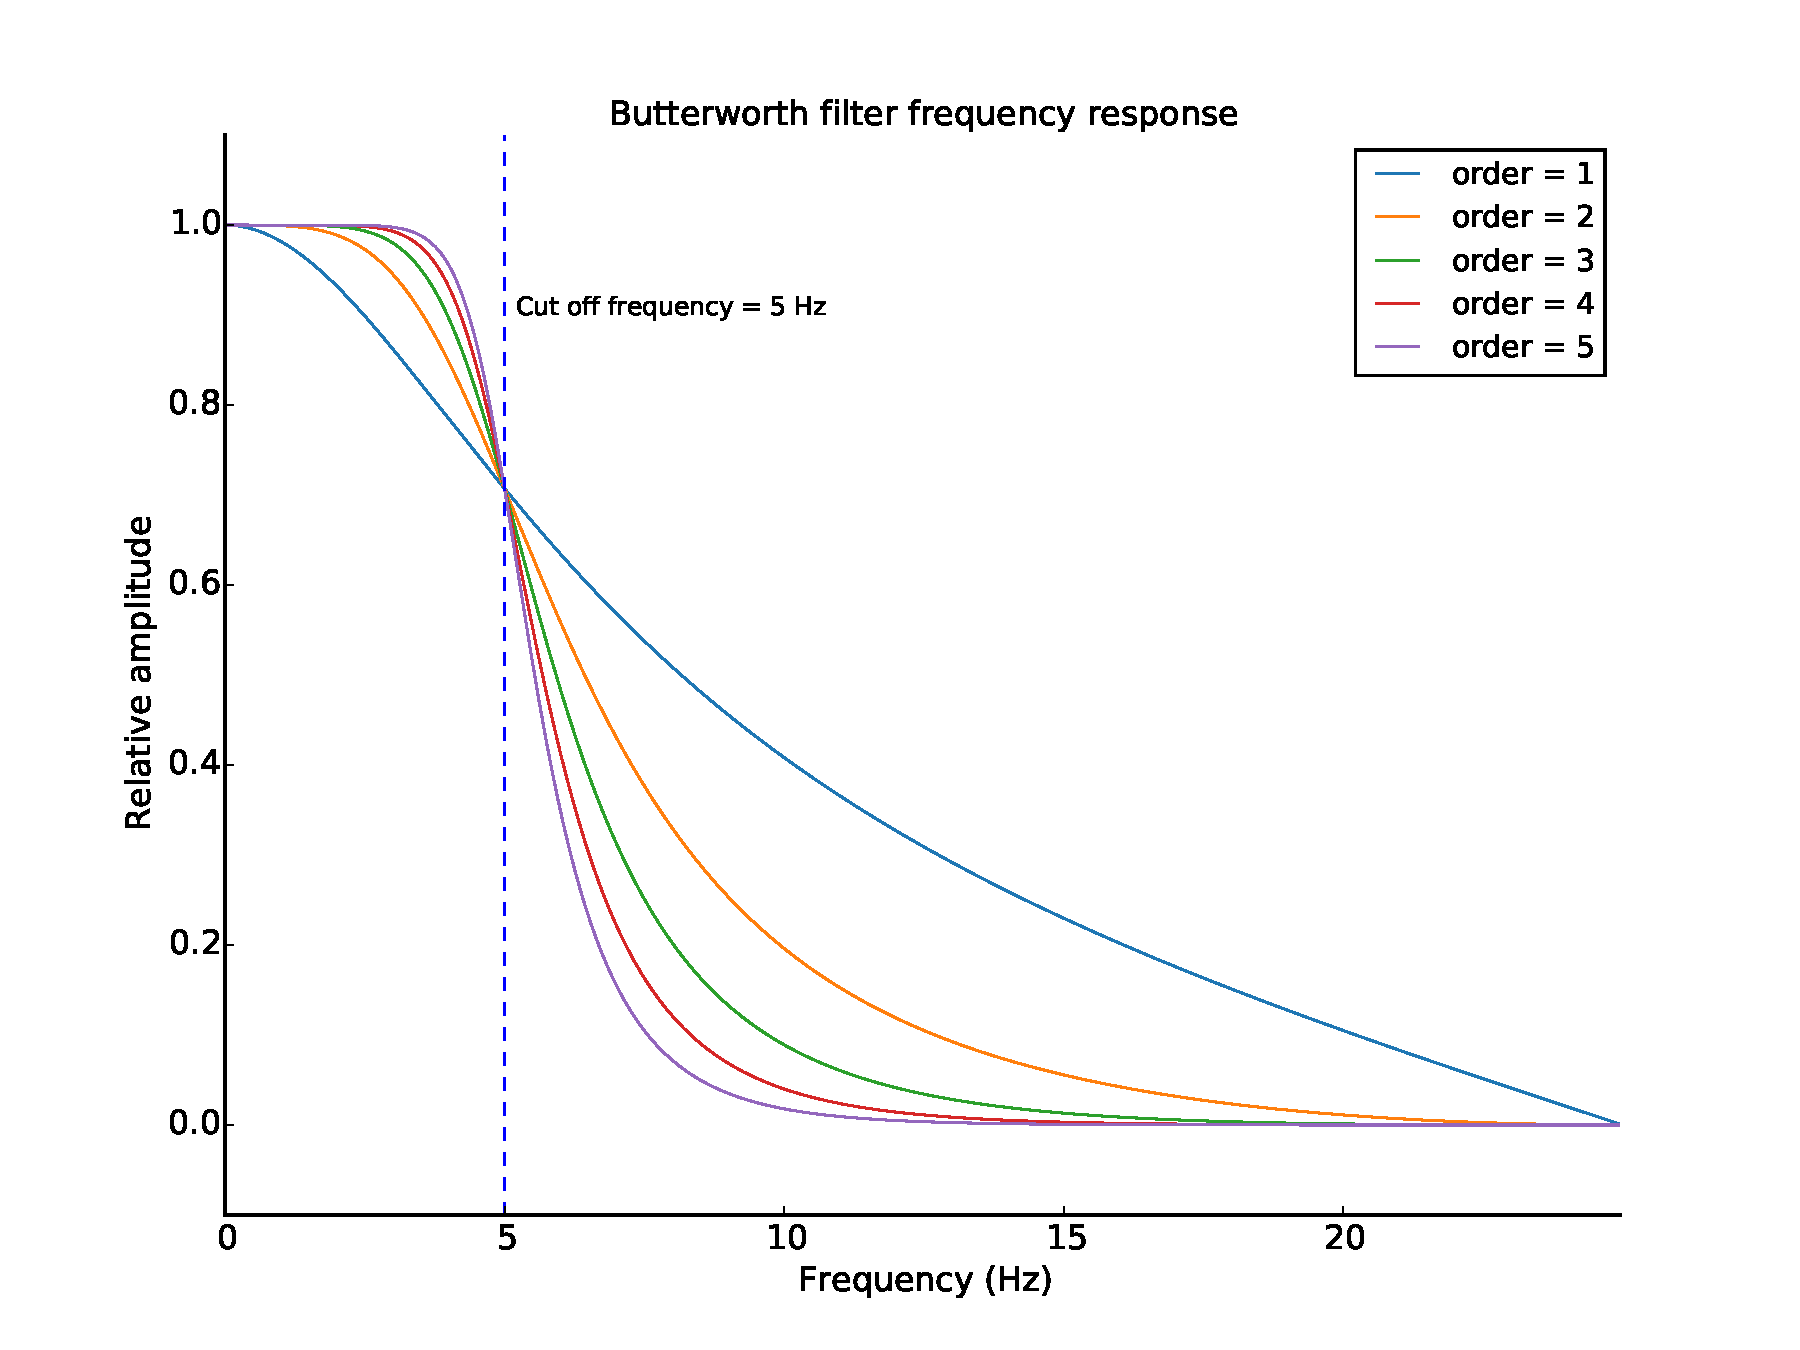
\includegraphics[width=1.0\textwidth]{butterworth_filters}
          \caption[Frequency response for Butterworth filters of different orders]{Frequency response for Butterworth filters of different orders. The higher the order, the quicker the cutoff between the pass band and the stop band. Each has a critical frequency of 5~\si{Hz}. At the critical frequency, the frequency response is equal to $\frac{1}{\sqrt{2}}$. A fifth-order Butterworth filter was used to filter the noise from the accelerometer data. }
          \label{fig:butterworth_filters}
        \end{figure}
        
        %disregard first and last 10 seconds
        %magnitude
        %filtering
      \subsubsection{Windows}
        Each data recording is split into 10 second windows, as in Hemminki \emph{et al.}\cite{hemminki2013accelerometer}. Features are extracted from each of these bins individually. Splitting into windows allows the production of multiple feature rows from the same recording. In theory, every window for a particular activity should exhibit extracted features that are consistent. A 10 second window was picked as a balance between producing enough feature rows from collected data and ensuring that several cycles of an activity were included. 
      
        %10 second overlapping bins
    \subsection{Feature extraction}
      \label{sec:feature-extraction}
      In total, 22 features are extracted from each window. The smartwatch and smartphone data are treated as separate windows for the purposes of feature extraction. This section goes on to describe and justify each of these features.
      
      \begin{table}
        \centering
        {\tabulinesep=1.2mm
        \begin{tabu} to \linewidth { c X[c]}
          \textbf{No of features} & \textbf{Description of each feature} \\
          \hline
          4 & Mean of each axis and magnitude \\
          4 & Standard deviation of each axis and magnitude \\
          4 & Maximum amplitude of each axis and magnitude \\
          4 & Median absolute deviation of each axis and magnitude \\
          3 & Pairwise correlation coefficient of each of the three axes \\
          1 & Spectral flatness of magnitude \\
          1 & Spectral entropy of magnitude \\
          1 & Frequency of maximum amplitude in the power spectrum of the magnitude \\
          \hline
        \end{tabu}}
        \caption{A summary of extracted features. A total of 22 features were extracted from the phone data, and another 22 features extracted from the watch data.}
        \label{tab:extracted-features}
      \end{table}
      
      \subsubsection{Mean of each axis and magnitude}
        The arithmetic mean $\bar{X}$ defined as $$\bar{X} = \frac{1}{n}\sum\limits_{i = 1}^{n}x_i$$ was calculated for each of the x, y and z axes and also for the magnitude.
        
        The arithmetic mean does not encode a lot of data, but is useful for determining primary orientation during the activity. For example, computer use has a z mean which is close to gravitational acceleration while the others are near zero. This indicates the devices primarily points upward during this activity.
      
      \subsubsection{Standard deviation of each axis and magnitude}
        The standard deviation $\sigma$ defined as $$\sigma = \sqrt{\frac{1}{n}\sum\limits_{i = 1}^{n}(\bar{x}-x_i)^2}$$ was calculated for each of the x, y and z axes and also for the magnitude.
        
        The standard deviation gives a measure of how much variation is present in each of the axes, and hence is useful when trying to recognise those activities that consistently have little variation in a particular measure. Gym cycling is one such activity, where the wrist moves comparatively little.
      \subsubsection{Maximum amplitude of each axis and magnitude}
        The maximum $x_{\max}$ defined as $$x_{\max} = \max_i x_i $$
        
        The maximum is a potentially useful figure but has the propensity to vary significantly between instances of the same activity. Another, perhaps more useful measure, would be the number of times the magnitude of the acceleration exceeds a certain threshold. 
      \subsubsection{Median average deviation of each axis and magnitude}
        The median average deviation $x_\mathrm{mad}$ is defined as $$x_\mathrm{mad} = \mathrm{median}_i (|x_i - \mathrm{median}_j(x_j)|)$$
        
        Though this measure follows the same trend as the standard deviation, its use of the median ensures it is a robust statistic --- one that is resistant to outliers --- and offers good performance on data that is not normally distributed. This is a desirable characteristic in activities such as fussball as recorded from the watch, as fussball requires gentle moves interspersed with quick movements with high acceleration.
      \subsubsection{Pairwise correlation coefficient for each of the three axes}
        The covariance is a measure of how much two random variables change together. The covariance of two random variables $X$ and $Y$, $\mathrm{Cov}(X, Y)$ is defined as $$\mathrm{Cov}(X, Y) = \mathbb{E}[(X - \bar{X})(Y - \bar{Y})]$$
        
        The correlation coefficient, $\mathrm{Cor(X,Y)}$, of two random variables $X$ and $Y$ is the normalised covariance of the two random variables. $$\mathrm{Cor(X,Y)} = \frac{\mathrm{Cov(X,Y)}}{\sigma_{\mathrm{X}}\sigma_{\mathrm{Y}}}$$
        
        $\mathrm{Cor(X,Y)}$ has a value between $-1$ and $1$, with $1$ representing total positive correlation, $0$ representing no correlation and $-1$ representing total negative correlation.
         
        The correlation coefficient was calculated for each pair of axes, producing three features: $\mathrm{Cor(X,Y)}$, $\mathrm{Cor(X,Z)}$, and $\mathrm{Cor(Y,Z)}$. The correlation coefficients give a measure of how much the axes move together during the recording. This encodes some information about the direction of movement.
      \subsubsection{Spectral flatness of magnitude}
        Spectral flatness is also known as the tonality coefficient. It is a measure of how noise-like or tone-like a signal is. White noise has spectral flatness approaching 1, while a pure tone has spectral flatness approaching zero.
        
        Spectral flatness is calculated from the power spectrum of the signal. Recall from Section~\ref{sec:intro-sig-processing} that the power spectrum is the squared magnitude of the Fourier transform of the signal.
        
        If $x_i$ represents the magnitude in the power spectrum of bin $i$, then the spectral flatness of a power spectrum $X = [x_1, x_2, \dots , x_N]$ is defined as
        
        $$\mathrm{Flatness(X)} = \frac{\sqrt[N]{\prod\limits_{i=1}^N x_i}}{\frac{1}{N}\sum_{i=1}^N x_i}$$
        
        The geometric mean can be expressed as a summation of logarithms rather than a product, giving an alternative formula for the spectral flatness that does not require a large product or an nth root. As the Fourier transforms in this project are likely to be over 10000 elements long, avoiding the large product or the expensive nth root calculation is desirable. Following conversion to a logarithmic summation, the spectral flatness is:
        
        $$\mathrm{Flatness(X)} = \frac{\exp \left( \frac{1}{N}\sum\limits_{i=1}^N \ln x_i \right) }{\frac{1}{N}\sum_{i=1}^N x_i}$$
        
        Spectral flatness gives a measure of how periodic a signal is. Activities where there is very high spectral flatness, akin to white noise, are aperiodic. For example, fussball and standing have no associated period, while walking has a clear period when measured through the smartphone.
      \subsubsection{Spectral entropy of the magnitude}
        The spectral entropy of a signal is calculated as the entropy of its power spectrum. It is defined as:

        $$\mathrm{entropy} = -\sum\limits_{i=1}^N x_i \log_2 x_i$$
        
        This feature is used successfully in Hemminki \emph{et al.}\cite{hemminki2013accelerometer} as a measure of how much information is present in its power spectrum.
        
      \subsubsection{Frequency of maximum amplitude in the power spectrum of the magnitude}
        The power spectrum of the magnitude shows the distribution of power in the frequencies of a signal. It is defined as the squared magnitude of the Fourier transform of the signal.
        
        Rather than take the Fourier transform of the original signal, the mean of the signal is first subtracted. If the original signal oscillates about some non-zero offset, the Fourier transform will have a spike at the origin (0 \si{Hz}, or the DC component). To avoid incorrectly classing 0 \si{Hz} as the maximum, the mean is subtracted from the original signal. The frequency of maximum amplitude of a power spectrum $X$ is then:
        
        $$\mathrm{f}_\mathrm{max} = \argmax_f X_f$$
        
        The frequency of maximum amplitude gives the principle frequency of the accelerometer data. For example, able-bodied people take between one and two steps in a second, and so we should expect a frequency of maximum amplitude in the $1 \sim 2 \si{Hz}$ range. Indeed, this is empirically what we see.
        
        A summary of the extracted features is given in Table~\ref{tab:extracted-features}.
    \subsection{Machine learning}
      Classification is supervised learning problem. This requires a classifier to be supplied with a set of instances, comprising sets of features, and a set containing a label for each instance. I use the following notation:
      \begin{itemize}
        \item a set of instances $X = \left\{X_1, X_2, \dots, X_N\right\}$ where each $X_i$ is a vector of $j$ features;
        \item a multiset of labels $y$ where $y_i \in \left\{1, 2, \dots, K\right\}$ is the label for instance $X_i$;
      \end{itemize}  
      
      This set of labelled instances is referred to as the \emph{training set}, which a classifier uses to generate a model. The classifier is then given a set of unlabelled instances, referred to as the \emph{test set}. The true labels of the test set are stored, but remain unknown to the classifier. The classifier generates a prediction for the test set, and a comparison between the predicted labels and the true labels forms the basis of any evaluative technique.
      
      I used four different classifiers:
      \begin{enumerate}
        \item Proportionally stratified random classifier (as a baseline)
        \item Naive Bayes classifier
        \item Decision Tree classifier
        \item Random Forest classifier
      \end{enumerate}
      
      I used implementations of these classifiers from Scikit Learn, though I explain the mechanisms below.
      
      \subsubsection{Proportionally stratified random classifier}
        The proportionally stratified random classifier acts as a dummy classifier. It randomly assigns labels to instances based on the proportion of the labels in the training set. This classifier is used to establish a baseline for evaluation.
        
        Thus, this classifier completely ignores all feature information. Given the training set, the classifier generates, for each $k \in \left\{1, 2, \dots, K\right\}$  a count $c_k$ of the number of times label $k$ appears in the set of labels $y$ i.e. the number of instances that are labelled $k$.
        
        Then during the test phase, the outputted label is in each case randomly selected. The probability of a label $k$ being output is $c_k / N$, where $N$ is the total number of instances in the training set.
        
        This classifier is only used to provide a baseline measurement against which we can compare other classifiers that do make use of the extracted features.
        
      \subsubsection{Naive Bayes classifier}
        The Naive Bayes classifier makes the naive assumption that all the features in the instance are independent. It then uses Bayesian probability to calculate the most probable class given the instance. 
        
        Mathematically we want to find $\mathbb{P}(y_k \mid X_i)$ for each label $y_k$ and each instance $\mathbf{X}_i$.
        
        \begin{flalign*}
          \mathbb{P}(y_k \mid \mathbf{X}_i) &= \mathbb{P}(y_k \mid x_1, x_2, \dots, x_j) &
          X_i \text{ is a vector of features} \\
          &= \frac{\mathbb{P}(y_k) \mathbb{P}(x_1, x_2, \dots, x_j \mid y_k)}{\mathbb{P}(\mathbf{X}_i)} &
          \text{Bayes' rule} \\
          &\propto \mathbb{P}(y_k) \mathbb{P}(x_1, x_2, \dots, x_j \mid y_k) &
          \mathbb{P}(X_i) \text{ is constant w.r.t. the label} \\
          &= \mathbb{P}(y_k) \mathbb{P}(x_1 \mid y_k) \cdots \mathbb{P}(x_j \mid y_k) &
          \text{Independence assumption} \\
          &= \mathbb{P}(y_k) \prod\limits_{i=1}^{j} \mathbb{P}(x_i \mid y_k) & \\
        \end{flalign*}
        
        % \begin{flalign*}
        % a_{11}& =b_{11}&
        % a_{12}& =b_{12}\\
        % a_{21}& =b_{21}&
        % a_{22}& =b_{22}+c_{22} \end{flalign*}

        The task then is to find the most probable label given the data: $$k = \argmax_k \mathbb{P}(y_k) \prod\limits_{i=1}^{j} \mathbb{P}(x_i \mid y_k)$$
      
        To calculate the probability of a particular continuous feature value $x_i$ given a label $y_k$, one can assume that the feature values follow a Gaussian distribution. Then, one can calculate the mean $\mu$ and the variance $\sigma^2$ for the value of the feature for a particular class.
      
        During the test phase, one can calculate the probability that $x_i$ takes its actual value $v$ given each of the classes using the equation for a normal distribution parameterised by $\mu$ and $\sigma^2$ for that particular class:
      
        $$\mathbb{P}(x_i = v \mid y_k) = \frac{1}{\sqrt{2 \pi \sigma^2}} \exp \left(-\frac{(v - \mu)^2}{2 \sigma^2}\right)$$
        
      \subsubsection{Decision Tree classifier}
        A decision tree classifier forms a tree where each node is a decision about a feature and labels appear as leaves.
        
        The training procedure for a decision tree classifier builds the tree recursively. For a node $m$, let $Q$ be the set of instance--label pairs in $m$. Create a possible split $\theta = (j, t)$ where $j$ is a feature and $t$ is some threshold value. Generate two subsets $Q_\mathrm{left}$ and $Q_\mathrm{right}$, where 
        $$Q_\mathrm{left}(\theta) = \left\{ (\mathbf{X}_i,y_i) \mid x_j <= t \right \}$$
        $$Q_\mathrm{right}(\theta) = Q \setminus Q_\mathrm{left} = \left\{ (\mathbf{X}_i,y_i) \mid x_j > t \right \}$$
      
        The impurity $G$ at $m$ is a measure of how far from a perfect dichotomy the split $\theta$ is for $Q$. The impurity $G$ requires an impurity metric $H$.
      
        $$G(Q, \theta) = \frac{|Q_\mathrm{left}(\theta)|}{|Q|} H(Q_\mathrm{left}(\theta)) + \frac{|Q_\mathrm{right}(\theta)|}{|Q|} H(Q_\mathrm{right}(\theta))$$
        
        
        
        There are two typical functions for the impurity metric $H$: the Gini impurity and the information gain. 
        
        The Gini impurity is given by:
      
        $$H(\mathbf{X}) = \sum \limits_{i=1}^K f_i(1-f_i) = 1 - \sum \limits_{i=1}^K f_i^2$$
      
        The information gain impurity is given by:
        $$H(\mathbf{X}) = \sum \limits_{i=1}^K f_i \log f_i$$
      
        where $f_i$ is the proportion of instances labelled $y_i$ in $\mathbf{X}$. Note that both the Gini impurity and the information gain impurity reach their minimum value, $0$, when $\mathbf{X}$ contains only a single class.
      
        The task then for the training phase of the decision tree classifier is to select the split $\theta^*$ that minimises the impurity:
      
        $$\theta^* = \argmin_\theta G(Q, \theta)$$
      
        The classifier then recursively repeats this process for $Q_\mathrm{left}$ and $Q_\mathrm{right}$ unless:
        \begin{itemize}
          \item $Q_\mathrm{left}$ or $Q_\mathrm{right}$ contain a single class, at which point they become a leaf node; or
          \item a pre-specified maximum depth has been reached; or
          \item the number of samples sent to the child node is less than a pre-specified minimum.
        \end{itemize}
      
        The introduction of a maximum depth and minimum sample size attempts to reduce the tendency for decision tree classifiers to overfit to the training data.
      
        The Scikit-Learn implementation of decision tree classifiers uses an optimised version of the CART (Classification and Regression Trees), developed by Breiman \emph{et al.}\cite{breiman1984classification}.
        
        A single CART model is easy to interpret, as it can be illustrated as a set of binary decisions. An extract of a decision tree classifier trained on phone and watch data can be seen in Figure~\ref{fig:decision-tree}.
        
        \begin{figure}
          \centering
          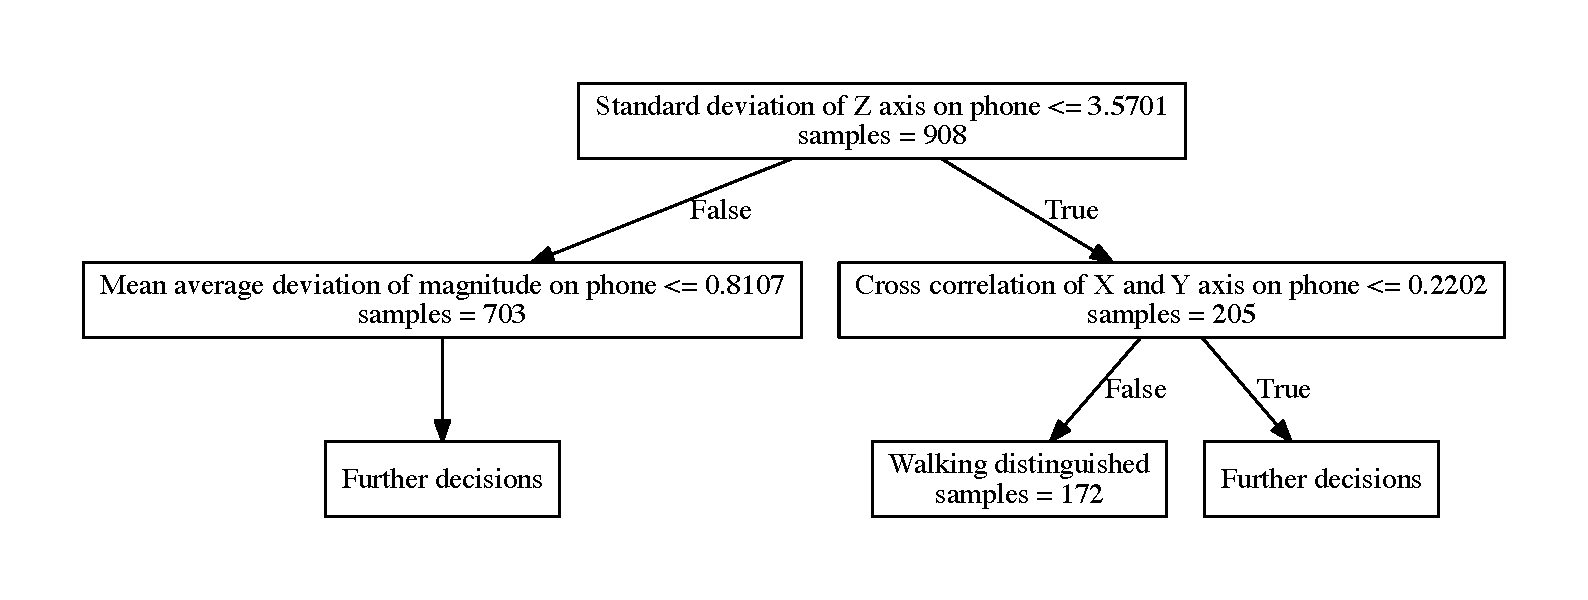
\includegraphics[width=1.0\textwidth]{bothtree}
          \caption[An extract of a decision tree classifier]{An extract of a decision tree trained on phone and watch data. Only two decisions are required to distinguish all walking samples in the training set.}
          \label{fig:decision-tree}
        \end{figure}
        
        The settings I used for the configuration of the decision tree -- known as hyperparameters -- I left at default settings. Optimising hyperparameters was ultimately unnecessary for accurate classification, and is dealt with partially by also using a random forest.
        
      \subsubsection{Random Forest classifier}
        The random forest classifier is an example of an ensemble classifier, one that makes use of a set of other classifiers. The random forest classifier that trains a collection of decision tree classifiers. Each decision tree classifier finds the best split from a random subset of features, rather than the absolute best split. The outputs from all the decision tree classifiers are then aggregated by the random forest classifier by outputting the modal label.
        
        Decision tree classifiers are prone to overfitting, especially when the are deep. The random forest classifier reduces variance by excluding different features from the training set, thus is less prone to overfitting.
        
        The cost of a random forest classifier over one single decision tree classifier is the increase in training time and memory requirements and also the loss interpretability of the resulting tree structure. The increased computational time required of a random forest classifier is not such a detriment in this offline processing task, but one might choose either a single decision tree or even a naive Bayes classifier if attempting to classify activities live.
        
        I kept most of the random forest hyperparameters at their default values except for the number of trees to use, which I increased from 10 to 50. More trees increases confidence in results.
  \section{Summary}
    In this section I have discussed:
    \begin{itemize}
      \item the backend and frontend components necessary to collect accelerometer data from the smartphone and smartwatch
      \item the activities I hope to be able to classify;
      \item how those activities have influenced the features I have extracted from the data;
      \item how four different classifiers use labelled instances of those features to classify new instances.
    \end{itemize}
